\section{System Architecture}\label{arch}

\subsection{Overview}
We revisit the architecture diagram in Figure \ref{sys-arch}, and formalize
the problems addressed in each one of the stages.

\vspace{0.5em}

\textbf{Featurization: } Formally, given a relation $R$ with a set of attributes $A$.
There is a featurization function $F$ which maps every row in $\mathcal{R}$ to a $d$ dimensional feature vector and a $l$ dimensional label tuple: 
\[F(r \in \mathcal{R}) \mapsto (\mathbb{R}^l, \mathbb{R}^d)\]
The result of the featurization are the data matrices $X$ and $Y$.
\[
F(R)\rightarrow (X,Y)
\]
The basic assumption is that training examples (i.e., rows in the data matrix) have a one-to-one relationship with rows in the base data ($R$).

\vspace{0.5em}

\textbf{Initialization: } To initialize \sys, the user gives us the base dirty relation $R$, the featurization $F$, and a model $\theta$ that is trained on this dirty relation.

\vspace{0.5em}

\textbf{Error Detection: } The first step in \sys is error detection. In this step, we select a candidate set of dirty records $R_{dirty} \subseteq R$. 

\vspace{0.5em}

\textbf{Error Sampling: } The second step in \sys is sampling. Since we cannot clean all of the dirty records, we take a sample of the records $S_{dirty} \subseteq R_{dirty}$.

\vspace{0.5em}

\textbf{Error Repair: } Next, we apply a repair procedure $C$ to the sample of data $S_{dirty}$ to get a clean sample $S_{clean}$.

\vspace{0.5em}

\textbf{Model Update: } Then, we update the model $\theta$ based on the newly cleaned data $F(S_{clean})$.

\vspace{0.5em}

\textbf{Error Impact Estimate: } Based on the change between $F(S_{clean})$ and $F(S_{dirty})$, we direct the next iteration of sampling to select points that will have changes most valuable to the model update.

\subsection{User Specified Steps}
\sys is a data cleaning methodology that iteratively corrects an incorrect result, and we formalize the conditions on the data cleaning operations that can fit in our framework.
The user has two specify two components: error detection and error repair.

\subsubsection{Error Detection}
We have to select a set of candidate records to be cleaned from the base data.
In our analysis, we assume that this candidate set is a superset of those records that are actually dirty.
Later, in Section \ref{imperfect}, we will relax this assumption.
Formally, given a relation $R$, we select a subset of records to be cleaned $R_{dirty}$.
Associated with each $r \in R_{dirty}$ is a set of errors $e_r$ which tells us which features are corrupted.
Therefore, the error detection step gives us the following tuple: $(R_{dirty},E_r)$.

\subsubsection{Error Repair}
Given a dirty record $r$, the error repair module applies a repair $C$ to the record, to return $C(r)\mapsto r_{clean}$. 

\iffalse


\subsubsection{Error Sampling}
Given a set of candidate dirty records, the error sampling step selects a sample to clean.
Records have to be sampled independently, i.e., sampling record $i$ does not affect the probability of sampling record $j$.
The input to this step is a sample size $K$ and the output is tuple of the a sample of $K$ records and their sampling probabilities.
The research problem that we explore in this work is how to construct this sampling distribution and feedback updates from the latest iteration.

\begin{problem}[Sampling Probability]\label{imp-samp}\sloppy
Given the current best model estimate $\theta$, data matrices $(X,Y)$, for each record $i$ calculate a sampling probability $p_i$.
\end{problem}

\subsubsection{Error Repair}
Given a set of sampled records, we apply data cleaning to this sample.
We define data cleaning as transformations that happens to the base data that result in changes to the feature vector. 
There is at most a one-to-one relationship between features in the cleaned data and the dirty data.
We require the following conditions on the data cleaning:
\begin{enumerate}
\item Single Operation. A dirty record is completely cleaned after applying the Error Repair module.
\item Persistence. Once cleaned there is no future operation that can invalidate the cleaning rendering the record dirty.
\item Sample-Local Write. The data cleaning must only modify the records in the sample.
\end{enumerate}
The output of this step are cleaned set of features vectors $\{(x_{clean},y_{clean})\}^K_i$.

\subsubsection{Incremental Model Update}
Given the sample of cleaned examples $\{(x_{clean},y_{clean})\}^K_i$ and the sampling probabilities, the next problem that we address is to update the model.

\begin{problem}[Incremental Update]\label{imp-update}\sloppy
Given the current best model estimate $\theta$, a clean sample $\{(x_{clean},y_{clean})\}^K_i$ , and a set of sampling probabilities $\{p\}^K_i$, we update the best model estimate from $\theta \rightarrow \theta'$.
\end{problem}

\subsubsection{Error Impact Estimate}
Once we compute $\theta'$, we feed this information back to update and guide the sampling distribution.
We want to calculate our sampling distribution with respect to the cleaned data, so for each remaining uncleaned record, we have an estimate of its cleaned value $(\hat{X},\hat{Y})$.
This estimate need not be very accurate as it is only used to select the sampling probabilities.

\begin{problem}[Error Impact Estimate]\label{imp-est}\sloppy
Let $(X_{dirty},Y_{dirty})$ be the data submatrices of the dirty data, $E_r$ be the error identifying set, and $(X_{clean},Y_{clean})$ be the submatrices for the cleaned data. Given $(X_{clean},Y_{clean})$, we learn a function $f$ that maps an $(x,y) \in (X_{dirty},Y_{dirty}) \mapsto (\hat{x},\hat{y})$.
\end{problem}
\fi

\subsection{Examples}
We illustrate how data cleaning processes proposed in the literature can apply in our model.
In particular, we describe how we can select a set of candidate records for cleaning and apply cleaning to the sample.

\subsubsection{Constraint-based Errors}
One model for handling errors in database declaring a set of constraints on a database and 
iteratively fixing records such that the constraints are satisfied \cite{DBLP:journals/pvldb/YakoutENOI11, DBLP:journals/pvldb/FanLMTY10, khayyat2015bigdansing}.
In this setting, it is relatively inexpensive to query the set of records that violate some constraint, however, automatically repairing the errors is often NP-Hard \cite{DBLP:journals/pvldb/FanLMTY10}.
Therefore, recently proposed systems like Guided Data Repair \cite{DBLP:journals/pvldb/YakoutENOI11}, use human input to validate suggested fixes.
The challenge with using human input is that it is expensive and is often with a time or a cost budget.
One way to characterize this problem setting is that error detection is relatively inexpensive but error repairing is expensive.

Formally, constraint-based error detection and repair can be incorporated into \sys in the following way.

\vspace{0.5em}

\noindent\textbf{Error Detection. } Let $\Sigma$ be a set of constraints on the relation $\mathcal{R}$. 
The allowed constraint classes are Matching Dependencies \cite{bertossi2013data}, Conditional Functional Dependencies \cite{DBLP:journals/pvldb/FanLMTY10}, and Denial Constrains \cite{khayyat2015bigdansing}. 
In the error detection step, we select a subset of records $\mathcal{R}_{dirty} \subseteq \mathcal{R}$ that violate at least one constraint.
The set $e_r$ the set of columns for each record which have a constraint violation.

\vspace{0.5em}

\noindent\textbf{Error Repair. } \sys supports both automated and human validated data repair for constraints. For automated techniques, we can apply the record-level ``local" repair proposed in \cite{DBLP:journals/pvldb/FanLMTY10} or we can use human corrections as in \cite{DBLP:journals/pvldb/YakoutENOI11}. Repair operations must satisfy the local property; that is, a repair to a record cannot cause additional constraint violations.

\begin{example}
Consider our EEG data running example, for an example of constraint-based cleaning.
We can add a constraint that one of the electrical signals cannot be greater than 4V.
For all records whose value is above 4V, we would select them in the error detection step.
Then, in the error repair step, we could apply a repair that sets the erroneous signal value to its most likely value.
\end{example}

\subsubsection{Value Filling}
Value filling is another data cleaning operation that is well studied in the literature.
Park and Widom proposed the system called CrowdFill \cite{park2014crowdfill}, where human workers fill in missing values in a database.

Formally, value filling error detection and repair can be incorporated into \sys in the following way.

\vspace{0.5em}

\noindent\textbf{Error Detection. } Let $\phi$ be the null-symbol (signifying a missing value), and $A$ be the set of attributes of $\mathcal{R}$. In the error detection step, we select a subset of records $\mathcal{R}_{dirty} \subseteq \mathcal{R}$ where $\mathcal{R}_{dirty}=\{r \in \mathcal{R}: \exists r(a\in A) = \phi \}$.
The set $e_r$ is the attributes of $r$ that have missing values.

\vspace{0.5em}

\noindent\textbf{Error Repair. } Value filling can be expressed in \sys if the operation fixes an entire record; that is, for all $a$ such that $r(a) = \phi$, a value is filled.

\begin{example}
Suppose, some of the patient information data is missing from dataset in our running example.
In the error detection step, we would select all of the records such there is a missing value.
In the error repair step, we could confirm that data with other records to fix the missing information.
\end{example}

\subsubsection{Entity Resolution}
Another common data cleaning task is Entity Resolution \cite{gokhale2014corleone, DBLP:journals/pvldb/KopckeTR10}.
In Entity Resolution, there is an attribute a in R such that $r(a)$ and $r'(a)$ refer to the same real-world entity but their representations are different $r(a) \ne r'(a)$.
Entity resolution typically consists of two steps: blocking and matching.
In the blocking step, similar records are grouped together, and in the matching step, they are resolved.
This process can be expressed in terms of a type of constraint called Matching Dependencies (described above).
A Matching Dependency (MD) is a constraint that if this pair is similar according to some similarity relationship (e.g., edit distance and a threshold) then their attribute have to be the same
\[ r \approx r' \implies r(a) \dot{=} r'(a) \]
Thus, this is an important special case of the constraint-based cleaning described before.

\vspace{0.5em}

\noindent\textbf{Error Detection. } Let $S$ be a similarity function that takes two records and returns a value in $[0,1]$ (1 most similar and 0 least similar). For some threshold $t$, $S$ defines a similarity relationship between two records $r$ and $r'$:
\[
r \approx r' : S(r,r') \ge t
\] 
In the error detection step, $R_{dirty}$ is the set of records that have at least one other record in the relation that satisfy $r \approx r'$.
The set $e_r$ is the attributes of $r$ that have entity resolution problems.

\vspace{0.5em}

\noindent\textbf{Error Repair. } \sys supports both automated and human validated entity resolution.

\begin{example}
An example of an Entity Resolution problem is where the patient's gender is inconsistently represented (e.g., ``Male", ``M", ``Man"). 
We can define a similarity relationship $(\text{first char =} 'M')$ and select all records that satisfy this condition.
In the error repair step, a human can fix the inconsistencies setting all records that meet the condition to the canonical value.
\end{example}

\iffalse

The cleaning operation $\mathcal{D}$ is a composition of $k$ ``cleaners":
\[
\mathcal{D}= C_{1} \circ C_{2} \circ ... C_{k}
\]
Each cleaner $C_i$ operates on a disjoint set of attributes of the relation R.

We study two models for these cleaners: Predicate and Learning.
In the predicate model, associated with each cleaner is a predicate $\rho_i$ that 
tells us which records are dirty and which are clean.
There are numerous real-world situations where detecting and enumerating errors are cheap but cleaning is expensive.
For example, if data is missing e.g., field misalignment it is often clear which rows are affected and which are not.
Similarly, in the entire field of constraint-based data cleaning \cite{nadeef}, we know in advance which records have constraint violations.
We can efficiently turn a set of functional dependencies into predicates so this model is compatible with data cleaning operations proposed in that field of work.

In the learning model, we assume nothing a priori about the data.
Associated with each cleaner is a classifier $\kappa_i$ that 
tells us which records are dirty and which are clean.
As we clean more data, we update the classifier.

\subsection{Problems}
We believe that interactive model building problem is best addressed by an anytime approach, where an analyst has a time budget and wants a best effort result given this time budget.
\sys optimizes the convergence of the model by adaptively changing the sampling distribution.
\sys is an optimizer that wraps around the SampleClean data cleaning library and Machine Learning libraries in Spark.
To achieve this, we have to address the following problems.

\begin{problem}[Importance Sampling Probability]\label{imp-samp}\sloppy
Given the current best model estimate $\theta$, data matrices $(X,Y)$, for each record $i$ calculate a sampling probability $p_i$ such that variance of the gradient step $\mathbb{E}(\|\nabla\phi\|_{2}^{2})$ is minimized.
\end{problem}

We will show that the optimal importance sampling distribution requires knowing the clean value of all the data, however, to a first-order, we can approximate it with estimates on already cleaned data.
We analyze the situation in which this estimate will reduce variance from the uniform sampling case where $p_i = p_j$.

Our algorithm is iterative where we sample data, update the model, and resample.
We also study the two model update problems:
\begin{problem}[Model Processing with Predicates]
Given an importance sampling distribution $p$ (from Problem \ref{imp-samp}), predicates $\{\rho\}_i$, and the model estimate $\theta$, update $\theta$ to $\theta'$.
\end{problem}

\begin{problem}[General Model Processing]
Given an importance sampling distribution $p$ (from Problem \ref{imp-samp}), classifiers $\{\kappa\}_i$, and the model estimate $\theta$, update $\theta$ to $\theta'$.
\end{problem}

\subsection{System Architecture}
In Figure \ref{sys-arch}, we illustrate our system architecture in contrast to a traditional data cleaning architecture to show how the above problems fit together.
Traditionally, data cleaning has explored expensive, up-front cleaning of entire datasets for increased accuracy on all possible queries.
Raw data is cleaned, then featurized, and then a model is trained based on the clean data.
In contrast, \sys explores a different architecture where data is progressively processed.
When we know the desired model in advance, we can feed this information back to guide and prioritize data cleaning.
In the process of fitting the model, we can integrate data cleaning rather than divorcing the two parts.

\subsection{Parameter Updates}
To achieve this architecture, \sys needs to maintain two states the parameter vector $\theta$ and the sampling distribution $P$.
We will formally describe the mathematics behind this process in the later sections.
In Figure \ref{param-arch}, we illustrate the structure of the parameter updates.
At each iteration, we draw a batch of dirty data using the sampling distribution $P$.
We calculate the average gradient for this data, and combine this gradient with the average gradient of the cleaned data.
We then update the parameter $\theta$ which in turn updates the sampling distribution.

\begin{figure}[t]
\centering
 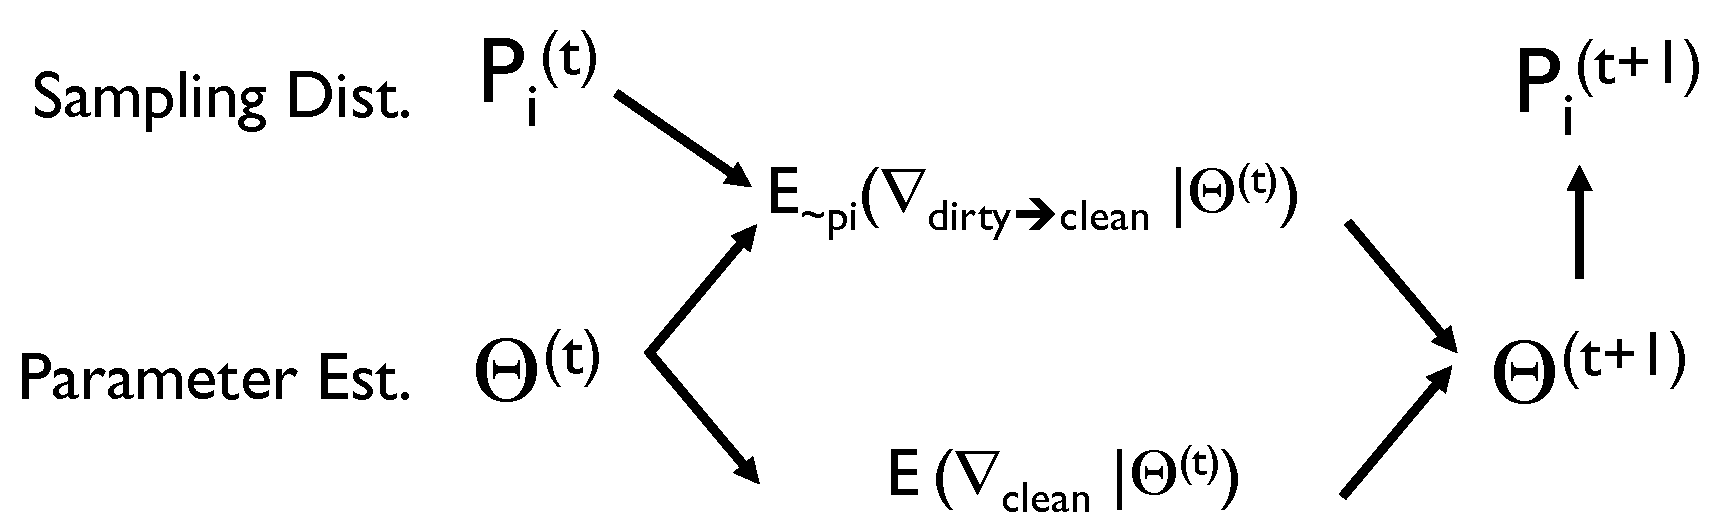
\includegraphics[width=\columnwidth]{figs/cmldag.pdf}
 \caption{The \sysfull operation DAG. At each iteration, we partition the data into clean and unknown quality. We fuse gradient estimates from the two partitions: (1) a sample from the unknown data using importance sampling, (2) a full (non-stochastic) gradient step on the clean data. After this estimate, we update the sampling distribution and the parameter.   \label{param-arch}}
\end{figure}



\subsection{Example Use Case And API}\label{api}
Consider the following example problem.
We are given the University of Texas Restaurant \footnote{http://www.cs.utexas.edu/users/ml/riddle/data/restaurant.tar.gz} dataset, which has the following schema:
\begin{lstlisting}[mathescape,basicstyle={\scriptsize}]
Restaurant(name$\textrm{,}$ address$\textrm{,}$ city$\textrm{,}$, type)
\end{lstlisting}
We want to train a Support Vector Machine classifier that given the tokens in the name and the city, can predict the category of the restaurant (e.g., Chinese or Mexican).
However, the challenge is that this dataset has numerous entity resolution problems where city names and categories are inconsistently represented.
\begin{lstlisting}[mathescape,basicstyle={\scriptsize}]
rex il ristorante,617 s. olive st.,los angeles,italian
rex il ristorante,617 s. olive st.,los angeles,nuova cucina italian
21 club,21 w. 52nd st.,new york,american
21 club,21 w. 52nd st.,new york city,american(new)
\end{lstlisting}
Entity resolution can be relatively expensive if the inconsistent representations are very different from each other and are not amenable to similarity measure optimizations such as prefix filtering or sorting.

\reminder{Maybe Describe API Here}

The analyst wants to quickly understand how much better a clean data set would be for this task.
Using our system, the analyst can construct a data cleaning workflow and specify a budget.
For example, this is what the code would look like in \sys.
\begin{lstlisting}[mathescape,basicstyle={\scriptsize}]
restaurant.load()

.clean(EntityResolution.weightedJaccard(`type',0.6))

.clean(EntityResolution.editDistance(`city',10))

.featureView(List(`type',`label'),(`city',`one_hot'),(`name',`bag_of_words')))

.model(new SVMModel(_))

.budget(5000)
\end{lstlisting}

\sys proposes an API for data cleaning pipeline construction. 
The API provides several data cleaning operations with known semantics.
Thus, we can use the lineage and operator semantics for optimization.
Of course, useful pipelines will often have User-Defined Functions and 
we will discuss the allowed operation types below.



\subsection{Algorithmic Problem Statement}
To formalize the optimization problem:

\noindent\textbf{Base Data and Featurization: } We are given a base dataset $\mathcal{R}$ which is a relation with $N$ rows. There is a featurization function $F$ which maps every row in $\mathcal{R}$ to a $d$ dimensional feature vector and a $l$ dimensional label tuple: \[F(r \in \mathcal{R}) \mapsto (\mathbb{R}^l, \mathbb{R}^d)\]. 

\noindent\textbf{Data Cleaning: } We define data cleaning as transformations that happens to the base data that result in changes to the feature vector. We do not consider data cleaning operations that change the number of rows in the relation such as row deletion or row deduplication. Allowed operations must result in the following changes to the feature vector: feature transformation and feature addition. Therefore, there is at most a one-to-one relationship beftween features in the cleaned data and the dirty data.

\reminder{Formalize Better}

\noindent\textbf{Budget Specification: } The analyst specifies two hyperparameters a cleaning budget $B$ which is the number of tuples to clean, and the number of cleaning rounds $T$. In each round, $\frac{B}{T}$ rows are processed by the system, we will discuss the tradeoffs between batching and incremental processing in the subsequent sections.

\reminder{Maybe exclude rounds}

\noindent\textbf{Model: } The analyst specifies the model which we require to be solved via convex regularized loss minimization:
\[
 \theta^{*}=\arg\min_{\theta}\sum_{i=1}^{N}\phi(x_{i},y_{i},\theta) + r(\theta)
\]

\noindent\textbf{Output: } The output of \sys is at each cleaning round we draw the sample of $\frac{B}{T}$ rows from a sampling distribution that incorporates information about the value of cleaning that row to model. After the $T$ cleaning rounds, the user is returned an approximately clean model $\theta^{(c)}$.
\fi
